
\documentclass[a4paper]{article}
\usepackage[utf8]{inputenc}
\usepackage[T1]{fontenc}     
\usepackage[francais]{babel}                        
\usepackage{tipa}
 \usepackage{textcomp}
\usepackage{graphicx}
\usepackage{array} % pour des tableaux particuliers                                                      
\usepackage[a4paper]{geometry}% Réduire les marges                         
\usepackage{multicol} % Pour faire plusieurs colonnes

	\usepackage{amssymb}
	\usepackage{mathrsfs}
	\usepackage{frcursive}
	\usepackage{color}

\usepackage{cite}

%\bibliographystyle{naturemag}



\title{Etat de l'art: "Apport des NGS pour inférer la structure de population"}      
\author{Pierre-Louis STENGER$^{1}$}




\date{}                       % La date n\textquotesingleest pas requise (la date du jour de compilation est utilisé en son absence)

\sloppy                       % Ne pas faire déborder les lignes dans la marge

\usepackage{amsmath,amssymb,amsthm,amsfonts}
\usepackage{nicefrac}

\DeclareMathOperator{\reff}{}

 % % % % % % % % % % % % % % % % % % % MARGES  % % % % % % % % % % % %  % % % % % % % % % % % % % % 
 
\setlength{\hoffset}{-18pt}         
\setlength{\oddsidemargin}{0pt} % Marge gauche sur pages impaires
\setlength{\evensidemargin}{9pt} % Marge gauche sur pages paires
\setlength{\marginparwidth}{54pt} % Largeur de note dans la marge
\setlength{\textwidth}{481pt} % Largeur de la zone de texte (17cm)
\setlength{\voffset}{-18pt} % Bon pour DOS
\setlength{\marginparsep}{7pt} % SÈparation de la marge
\setlength{\topmargin}{0pt} % Pas de marge en haut
\setlength{\headheight}{13pt} % Haut de page
\setlength{\headsep}{10pt} % Entre le haut de page et le texte
\setlength{\footskip}{27pt} % Bas de page + sÈparation
\setlength{\textheight}{708pt} % Hauteur de la zone de texte (25cm)


 % % % % % % % % % % % % % % % % % % % FOND GRIS  % % % % % % % % % % % % % % % % % % % % % % % % % 

\usepackage{amssymb,amscd,latexsym,amsmath,amstext}
\usepackage{xkeyval}
\usepackage{framed}
\usepackage{xcolor}
\usepackage{fancybox}
\usepackage{multido}
\newlength{\DSFBox}
\newlength{\SSFBox}
\newlength{\DEFBox}
\newlength{\EFBox}
\makeatletter
\define@key{BCouleur}{ctexte}{\def\CTexte{#1}} % Couleur du texte
\define@key{BCouleur}{cbord}{\def\CBord{#1}} % Couleur du bord
\define@key{BCouleur}{cfond}{\def\CFond{#1}}   % Couleur du fond
\define@key{BCouleur}{sfbox}{\def\SFBox{#1}}        % pour \fboxsep
\define@key{BCouleur}{epaisfbox}{\def\EpaisFBox{#1}} % pour \fboxrule
% par dÈfaut
\setlength{\DSFBox}{5pt}
\setlength{\DEFBox}{3pt}
\setkeys{BCouleur}{ctexte=black,cbord=gray!20,cfond=gray!20,sfbox=\the\DSFBox,
epaisfbox=\the\DEFBox}{}
\newenvironment{BCouleur}[1][]{%
\setkeys{BCouleur}{#1}
  \def\FrameCommand{\fboxrule=\FrameRule \fboxsep=\FrameSep \color{\CTexte}\fcolorbox{\CBord}{\CFond}}
\setlength{\SSFBox}{\SFBox}
\setlength\FrameSep{\the\SSFBox}
  \setlength{\EFBox}{\EpaisFBox}
\setlength\FrameRule{\the\EFBox}
  \MakeFramed{\advance\hsize-\width \FrameRestore}}%
  {\endMakeFramed}
\makeatother

% % % % % % % % % % % % % % % % % % % % % % % % % % % % % % % % % % % % % % % % % % % % % % % % % 



\begin{document}
	
\vspace*{\stretch{1}}
\begin{cursive}
\textbf{In the beginning there was nothing.
\\
God said: 'Let there be light !'
\\
There was still nothing, but now you could see it.
\\
(Dave Thomas)}
\end{cursive}
\vspace*{\stretch{1}}	

\newpage

\maketitle     
                                                   
$^{1}$Université de La Rochelle, Master 2 Gestion de l'Environnement et Ecologie Littorale (GEEL)

\begin{BCouleur}  % Début fond gris


\begin{abstract}
Résumé
\end{abstract}


\end{BCouleur} % Fin fond gris

\textbf{Key words:} \textit{NGS, Population, Génétique}

\section*{Introduction}      

\section{Mémo notes}

Apport des NGS pour inférer la structure de population

--> Qu'est ce que ça nous apprend de plus ?

Méthodes traditionnelles en génétiques des populations --> Dérive, mutation et migration. --> "On était bien" BSB\copyright

NGS ont permis de prendre en compte la sélection et ça à mis 30 ans de recherches en question.

~Basin (2006) --> Taille de la population décorrélé au nombre de diversité mitochondriale --> Il faudrait faire un balayage sélectif
~~\\
RAD SEQ --> Moins de marqueur que 454
Amélia --> Dauphin commun --> Structure population en Atlantique --> Augmentation du nombre de marqueur --> Augmentation de la puissance statistique
Car génétique ne montrait qu'une seule population, alors que écotoxicologie et isotopes en montraient plusieurs.
On va travailler sur marqueur de sélection --> Adaptation locale --> Ce sont les marqueurs Outlayer --> FST --> Avec les FST on revient dans un système circulaire (on a deux populations, on veut les différencier, on a un FST, on regarde si c'est supérieur. Aurait-on le même résultats avec 5 population ? Si on a 1000 marqueurs, il y en a forcement --> Statistiques fréquentistes (c'est à l'opposé des statistiques bayésiennes))
--> On coupe le jeu de données en deux.
~~\\
Do it yourself ABC (Marie Louis, usé à la fin de thèse)
--> Histoire évolutive
~~\\
Eric: 
\begin{itemize}
\item Séquenceur nanoport (Oxford)
\item Micness --> Séquence en NGS les microsatelites, Marie Suez et al. 2015
\end{itemize}

Séquenceur à plaques --> N'est pas un NGS

\section{A creuser}

http://www.sciencemag.org/content/312/5773/570.short --> E. Bazin, S. Glemin, N. Galtier, Science 312, 570 (2006).

Au sein des espèces, la diversité génétique est pensée pour refléter la taille de la population , l'histoire , l'écologie et capacité d'adaptation. Avec l'utilisation d'une collection complète d'ensembles de données de polymorphisme couvrant ~3000 espèces animales , Bazin et al (2006) montrent que l'ADN mitochondrial (ADNmt) est un marqueur couramment utilisé quui ne reflète pas l'abondance des espèces ou de l'écologie : la diversité ADNmt n'est pas plus élevé chez les invertébrés que chez les vertébrés , en milieu marin que dans chez les espèces terrestres, ou que dans les petits organismes par rapport aux grands. Le loci nucléaire, en revanche, est adapté à ces attentes intuitives. La distribution inattendue de la diversité mitochondrial est expliquée par l'évolution adaptative récurrente, contestant la théorie neutraliste de l'évolution et de remettre en question la pertinence de l'ADNmt dans les études de la biodiversité et de conservation.

~~\\
Thèse HDR de Didier AURELLE:

La majorité des études de génétique des populations réalisées jusqu'à présent sont faites sous l'hypothèse d'une évolution neutre ou quasi neutre des marqueurs employés. Or d'une part la neutralité de divers marqueurs couramment utilisés peut être remise en cause qu'il s'agisse de l'ADN mitochondrial (Bazin et al., 2006) ou des microsatellites (Kashi et King, 2006). D'autre part l'étude de l'impact des changements environnementaux et notamment du changement global sur les populations naturelles nécessite de prendre en compte les processus sélectifs, ou au moins de se poser la question des capacités d'évolution des organismes par rapport à la vitesse de ces changements (Berteaux et al., 2004) et donc de s'intéresser à la diversité génétique adaptative et à ses relations avec la diversité neutre.


~~\\

Via Thèse HDR de Didier AURELLE: Calderón I., Garrabou J., Aurelle D. (2006) Evaluation of the utility of COI and ITS markers as tools for population genetic studies of temperate gorgonians. Journal of Experimental Marine Biology and Ecology, 336, 184-197. doi:10.1016/j.jembe.2006.05.006.:


L'ADN mitochondrial présente des propriétés qui en font a priori un marqueur de choix pour une étude de phylogéographie: généralement pas de recombinaison, un taux de dérive plus important que l'ADN nucléaire et un niveau élevé de polymorphisme (Avise, 2000). Cependant comme l'ont noté Ballard et Whitlock (2004) ses propriétés biologiques peuvent aussi représenter des inconvénients: il ne reflète que l'histoire des lignées maternelles et l'absence de recombinaison associée à la forte densité en gènes le rend aussi plus sensible à la perte de variabilité suite aux fixations de mutations avantageuses ("genetic draft"; Bazin et al., 2006). Malgré tout, ce marqueur permet de fournir une première image de la structuration génétique d'une espèce sous réserve de garder à l'esprit les contraintes précédentes.

~~\\

Review de l'article Bzin et al. 2006: Kitchen, A., Miyamoto, M. M., & Mulligan, C. J. (2008). A three-stage colonization model for the peopling of the Americas. PLoS One, 3(2), e1596.

Bazin et al . (Rapports, le 28 avril 2006 , p . 570 ) n'a trouvé aucune relation entre ADNmt diversité et la taille de la population lorsque l'on compare entre grands groupes d'animaux . Nous montrons empiriquement que les espèces avec de petites populations , telle que représentée par les mammifères euthériens , présentent une corrélation positive entre l'ADNmt et variation des allozymes , ce qui suggère que la diversité peut ADNmt corrélation avec la taille de la population de ces animaux.

~~\\
Do it yourself: Thèse Marie Louis Chapitre 6, page 162:

We investigated the demographic history best describing the genetic dataset of the combined microsatellite and mtDNA markers using a coalescent-based Approximate Bayesian Computation (ABC) approach (Beaumont et al. 2002; Bertorelle et al. 2010; Csilléry et al. 2010, the general principle of this analysis is presented in Chapter 2.2c).

~~\\

RAD Seq Amélia:

Amélia Viricel, Eric Pante, Willy Dabin, Benoit Simon-Bouhet. Applicability of RAD-tag geno- typing for inter-familial comparisons: empirical data from two cetaceans. Molecular Ecology Resources, Blackwell, 2014, 14 (3), pp.597-605. <10.1111/1755-0998.12206>. <hal-00908459>

Viricel, A., & Rosel, P. E. (2014). Hierarchical population structure and habitat differences in a highly mobile marine species: the Atlantic spotted dolphin. Molecular ecology, 23(20), 5018-5035.

~~\\

blabla \cite{Sanchez20161} blabla

blabla \cite{Lane:2016aa}

\section{Historique des technologies}

\begin{itemize}
\item 1953: Découverte de la molécule d'ADN par Watson et Crick
\item 1973: Première séquence de 24 paires de bases publiée (Walter Gilbert and Allan Maxam 1973. The nucleotide sequence of the lac operator)
\item 1975: Southern Blot
\item 1977: Séquençage Sanger & Gilbert
\item 1982: Genbank started
\item 1983: Developpement des PCR (Polymerase Chain Reaction)
\item 1987: Premier sequenceur automatique: Applied Biosystems Prism 373
\item 1990: Séquençage par mesure de la fluorescence
\item 1995: Puces à ADN (microarray)
\item 1996: Sequenceur à capillaires: ABI 310
\item 1998: Genome de \textit{Caenorhabditis elegans} séquencé
\item 2000: Evolution des puces à ADN
\item 2003: Séquençage du génome humain. ~3 milliards de dollars, 13 ans 
\item 2005: 1st 454 Life Sciences Next Generation Sequencing system : GS 20 System
\item 2006 : 1st Solexa Next Generation Sequencer : Genome Analyzer
\item 2007 : 1st Applied Biosystems Next Generation Sequencer : SOLiD
\item 2007: Séquençage d'un individu (JC Venter) Méthode Sanger (Levy et al. Plos Bio 2007)
\item 2008: Séquençage d'un individu (J.D Watson) Méthode haut débit (454 Roche) (Wheeler et al. Nature 2008), 1 million de dollar, 2 mois
\item 2009 : 1st Helicos single molecule sequencer : Helicos Genetic Analyser System 2011 : 1st Ion Torrent Next Generation Sequencer : PGM
\item 2011 : 1st Pacific Biosciences single molecule sequencer : PacBio RS Systems
\item 2012 : Oxford Nanopore Technologies demonstrates ultra long single molecule reads
\item 2012: "Next-next generation Sequencing"
\end{itemize}

\begin{figure}[!h]
\centering{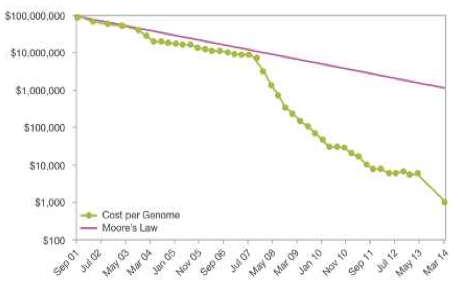
\includegraphics[scale=0.5]{evolution}}
\caption{Evolution très rapide des instruments, des débits et des coûts (premier séquençage sur 454 en Janvier 2008)}
\end{figure}

~~\\

10 ans --> Prix divisé par 100 000

\section{Définition NGS}

NGS --> Séquençage à haut débit, Next Generation Sequenching, NextGen Sequencing, NGS, Massively Parallel Sequencing

\section{Grands principes NGS}

Sanger: 96 ADNs différents analysés en une fois
NGS: Millions d'ADNS différents analysés en une fois 
--> Saut technologique

\begin{itemize}
\item Intégration (système combinant les avantages de la PCR et des puces)
\item Parallélisation (PCR multiplex)
\item Miniaturisation
\end{itemize}

NGS à permis le séquençage entier du génome humain --> Wheeler, D. A., Srinivasan, M., Egholm, M., Shen, Y., Chen, L., McGuire, A., ... & Gomes, X. (2008). The complete genome of an individual by massively parallel DNA sequencing. nature, 452(7189), 872-876.

~~\\ 
Voelkerding 2010
Matériel biologique: ADN ou ARN
Etapes communes aux différentes technologies:
\begin{itemize}
\item Fragmentation enzymatiques de l'ADN
\item Préparation d'une banque (library) par ligation d'adaptateurs
\item Amplification clonale
\item Séquençage générant des signaux (luminescent ou fluorescent)
\item Détection des signaux émis et conversion en séquence
\end{itemize}

\begin{figure}[!h]
\centering{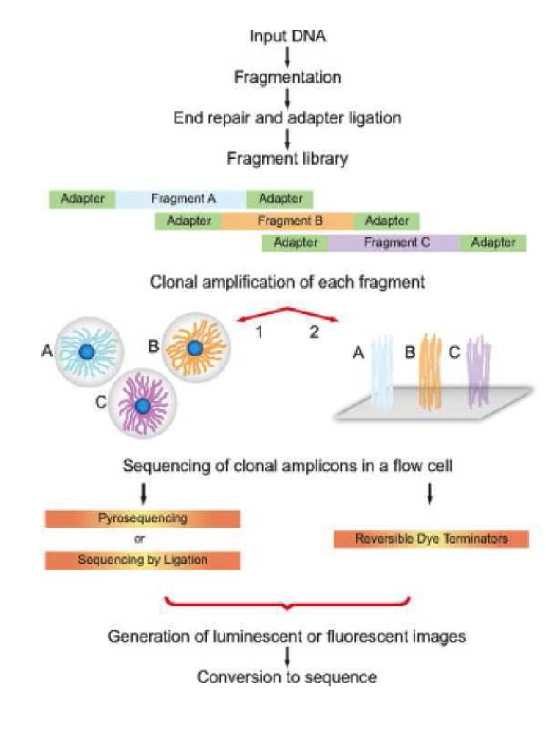
\includegraphics[scale=0.5]{principes}}
\caption{Grands principes NGS}
\end{figure}

\begin{figure}[!h]
\centering{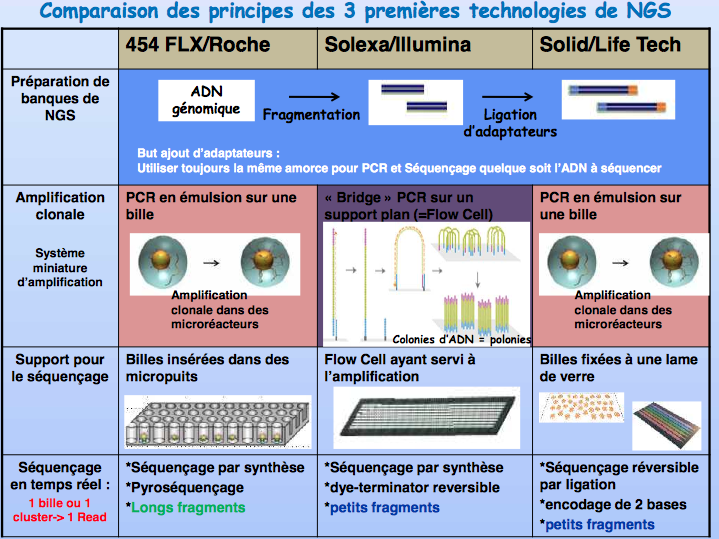
\includegraphics[scale=0.5]{comparaison2}}
\caption{Comparaison des principes des trois premières technologies de NGS}
\end{figure}


\begin{figure}[!h]
\centering{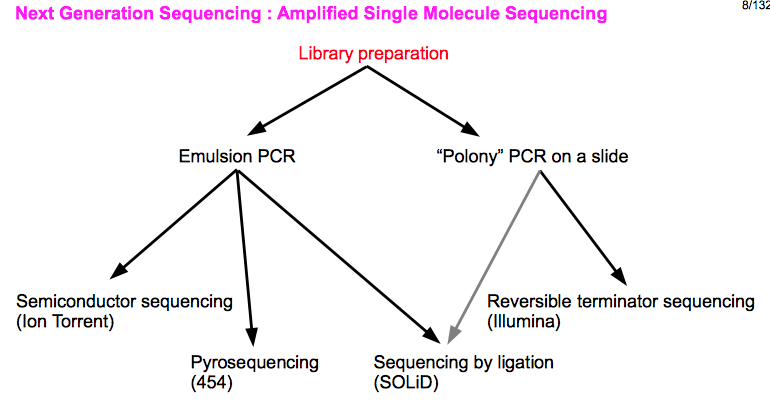
\includegraphics[scale=0.5]{ASMS}}
\caption{Next Generation Sequencing, Amplified Single Molecule Sequencing}
\end{figure}

\section{Library preparation}

\section{Emulsion PCR}

\section{"Polony" PCR on a slide}

\section{Les différentes plateformes (Sommaire)}


\underline{454 Sequencing / Roche:(1)}
\begin{itemize}
\item GS Junior System
\item GS FLX+ System 
\end{itemize}

\underline{Illumina (Solexa)(1):}
\begin{itemize}
\item HiSeq System 
\item Genome analyzer IIx 
\item MySeq
\end{itemize}

\underline{Applied Biosystems - Life Technologies:(1)}
\begin{itemize}
\item SOLiD 5500 System
\item SOLiD 5500xl System
\end{itemize}

\underline{Ion Torrent - Life Technologies:(1)}
\begin{itemize}
\item Personal Genome Machine (PGM)
\item Proton
\end{itemize}

\underline{Helicos:(2)}
\begin{itemize}
\item Helicos Genetic Analysis System 
\end{itemize}

\underline{Pacific Biosciences:(2)}
\begin{itemize}
\item PacBio RS
\end{itemize}

\underline{Oxford Nanopore Technologies:(2)}
\begin{itemize}
\item GridION System 
\item MinION
\end{itemize}

~~\\

(1) = Next Generation Sequencing, Amplified Single Molecule Sequencing

~~\\

(2) = Third Generation Sequencing, Next Next Generation Sequencing, Single Molecule Sequencing

~~\\


\begin{figure}[!h]
\centering{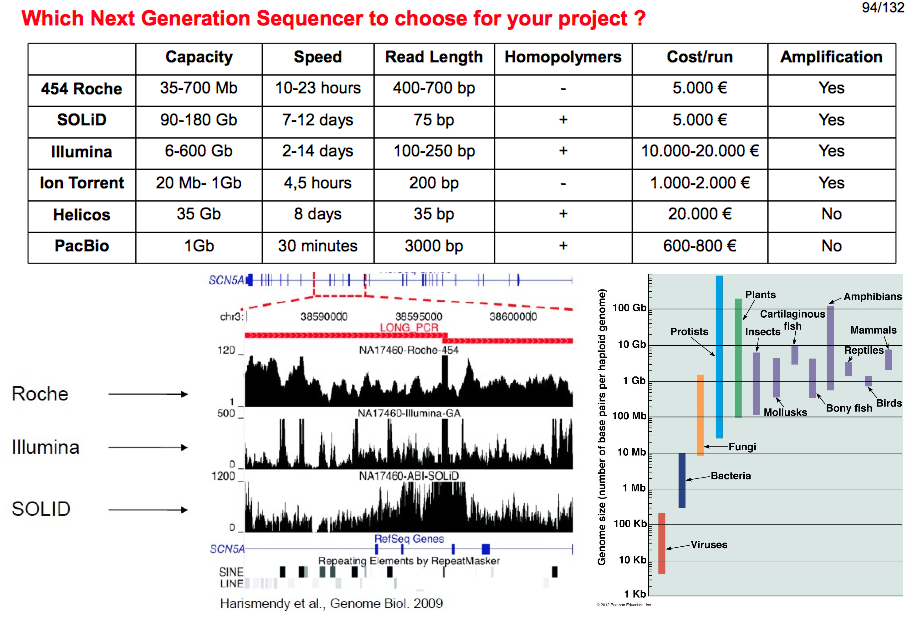
\includegraphics[scale=0.5]{bla}}
\caption{Que choisir ?}
\end{figure}

\begin{figure}[!h]
\centering{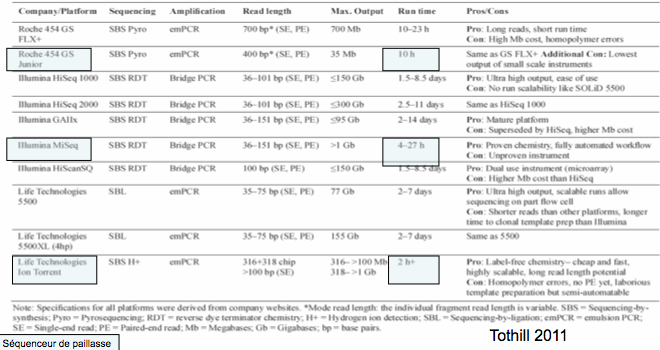
\includegraphics[scale=0.5]{comparaison}}
\caption{Comparaison NGS}
\end{figure}


\section{454 Sequencing/ Roche}
 
\begin{figure}[!h]
\centering{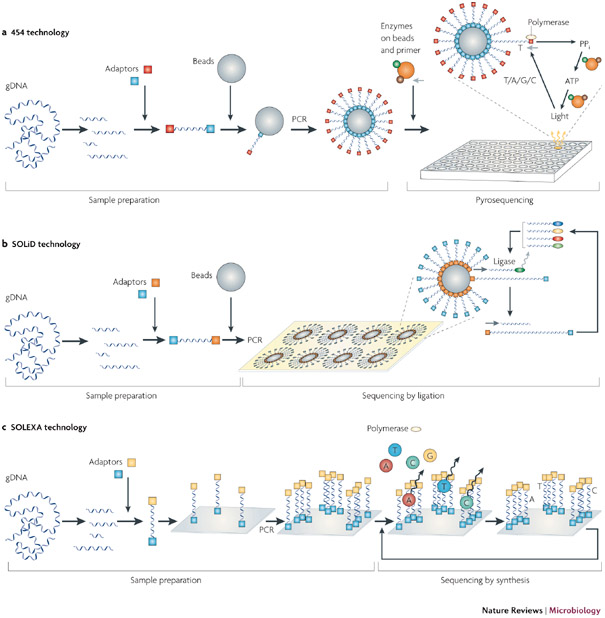
\includegraphics[scale=0.5]{454}}
\caption{Plusieurs méthodes}
\end{figure}


\begin{figure}[!h]
\centering{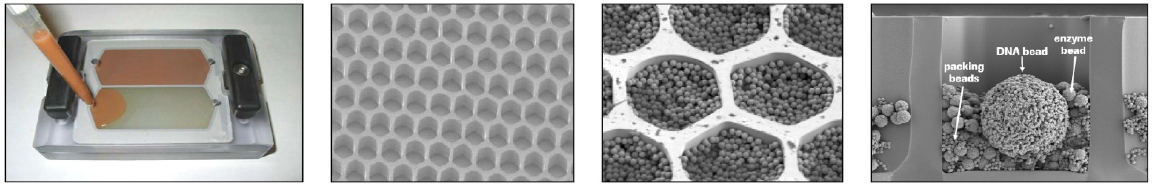
\includegraphics[scale=0.5]{sequencage454}}
\caption{sequencage454}
\end{figure}

\subsection{GS Junior System}

\subsection{GS FLX + System}

\section{Illumina}

\subsection{HiSeq System}

\subsection{Genome analyser IIX}

\subsection{MySeq}

\section{Applied Biosystems - Life Technologies}

\subsection{SOLiD 5500 System}

\subsection{SOLiD 5500xl System}

\section{Ion Torrent}

Particularités :
\begin{itemize}
\item Pas de système optique
\item Support de séquençage = surface semi-conducteur 
\item Mesure du pH (ion H+ produit par l’ADN polymerase lors de l’incorporation de chaque base)
\end{itemize}

Erreurs de séquençage récurrentes spécifiques comme des erreurs dans les homopolymers -> indels artefactuels

\subsection{Personal Genome Machine (PGM)}

\subsection{Proton}

\section{Next nexte gen:}

\begin{itemize}
\item Séquençage sur molécule unique
\item Pas d'amplification clonale
\item Inconvénient actuel: Taux élevé d'erreurs de séquences (taux d'erreur de séquençage 10 fois plus élevé qu'avec le séquençage Sanger selon http://www.math-info.univ-paris5.fr/~rozen/Analyse-Genome-Tumoral/Exposes%202014/Christine-BOLE-FEYSOT.pdf)
\end{itemize}

\section{Helicos}

\subsection{Helicos Genetic Analysis System}

\section{Pacific Biosciences}

\subsection{PacBio RS}

\section{Oxford Nanopore Technologies}


\begin{figure}[!h]
\centering{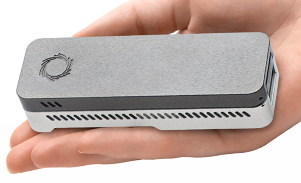
\includegraphics[scale=0.5]{Nanoport}}
\caption{Nanoport}
\end{figure}

\begin{figure}[!h]
\centering{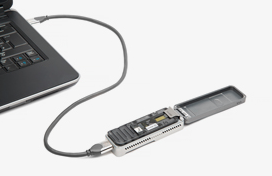
\includegraphics[scale=0.5]{Nanoport2}}
\caption{Nanoport}
\end{figure}

\begin{figure}[!h]
\centering{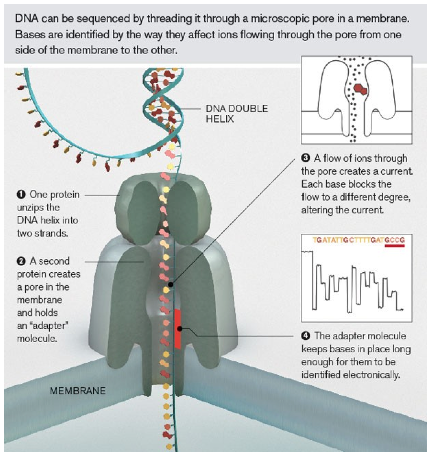
\includegraphics[scale=0.5]{nano}}
\caption{Nanoport}
\end{figure}

MinION & PromethION

Hargreaves and Mulley (2015), Assessing the utility of the Oxford Nanopore MinION for snake venom gland cDNA sequencing. PeerJ 3:e1441; DOI 10.7717/peerj.1441
--> "Le MinION deviendra l'approche par défaut du séquençage d'ADN circulaire dans la variété des espèces"

Une plaque 900 dollars
48 plaques 24 00 dollars

\subsection{GridION System}

\subsection{MinION}



\section{MicNeSs}

Suez, M., Behdenna, A., Brouillet, S., Graça, P., Higuet, D. and Achaz, G. (2015), MicNeSs: genotyping microsatellite loci from a collection of (NGS) reads. Molecular Ecology Resources. doi: 10.1111/1755-0998.12467
~~\\
Les microsatellites sont largement utilisés dans la génétique des populations pour découvrir événements évolutifs récents. Ils sont généralement génotypés en utilisant un séquenceur à capillaire, dont la capacité est généralement limitée à 9, au plus 12 loci pour chaque terme, et dont l'analyse est une tâche fastidieuse qui est effectué à la main. Avec la montée de séquençage de nouvelle génération (NGS), un plus grand nombre de lieux et de personnes sont disponibles à partir de séquençage: par exemple, sur un seul passage d'un GS junior, 28 loci de 96 personnes sont séquencées avec une couverture 30X. Suez et al 2015 ont développé un algorithme pour génotyper automatiquement et efficacement les microsatellites à partir d'un recueil de lectures triés par individu (par exemple amplifications par PCR spécifiques d'un locus ou d'une collection de lit qui englobent un locus d'intérêt). Comme le séquençage et l'amplification par PCR introduisent des insertions ou délétions artefactuelles, l'ensemble de lit à partir d'un seul allèle microsatellite montre plusieurs variantes de longueur. Les déduits de l'algorithme, sans alignement, la vraie inconnue allèle (s) de chaque individu à partir des distributions observées de microsatellites longueur de tous les individus. MicNeSs, une implémentation de Python de l'algorithme, peut être utilisé pour le génotype toute locus microsatellite de tout organisme et a été testé sur 454 données de pyroséquençage de plusieurs loci de mouches des fruits (espèce de modèle) et cerfs rouges (espèce nonmodel). Sans aucune parallélisation, il génotype automatiquement 22 loci de 441 personnes en 11 heures sur un ordinateur standard. La comparaison des inférences MicNeSs la méthode standard montre un excellent accord, avec quelques différences illustrant les avantages et les inconvénients des deux méthodes.


\section{Les limitations des NGS}

PDF NGS


\listoffigures  % table des figures
\listoftables   % table des tableaux

\section*{ANNEXE: Emulsion}


\begin{figure}[!h]
\centering{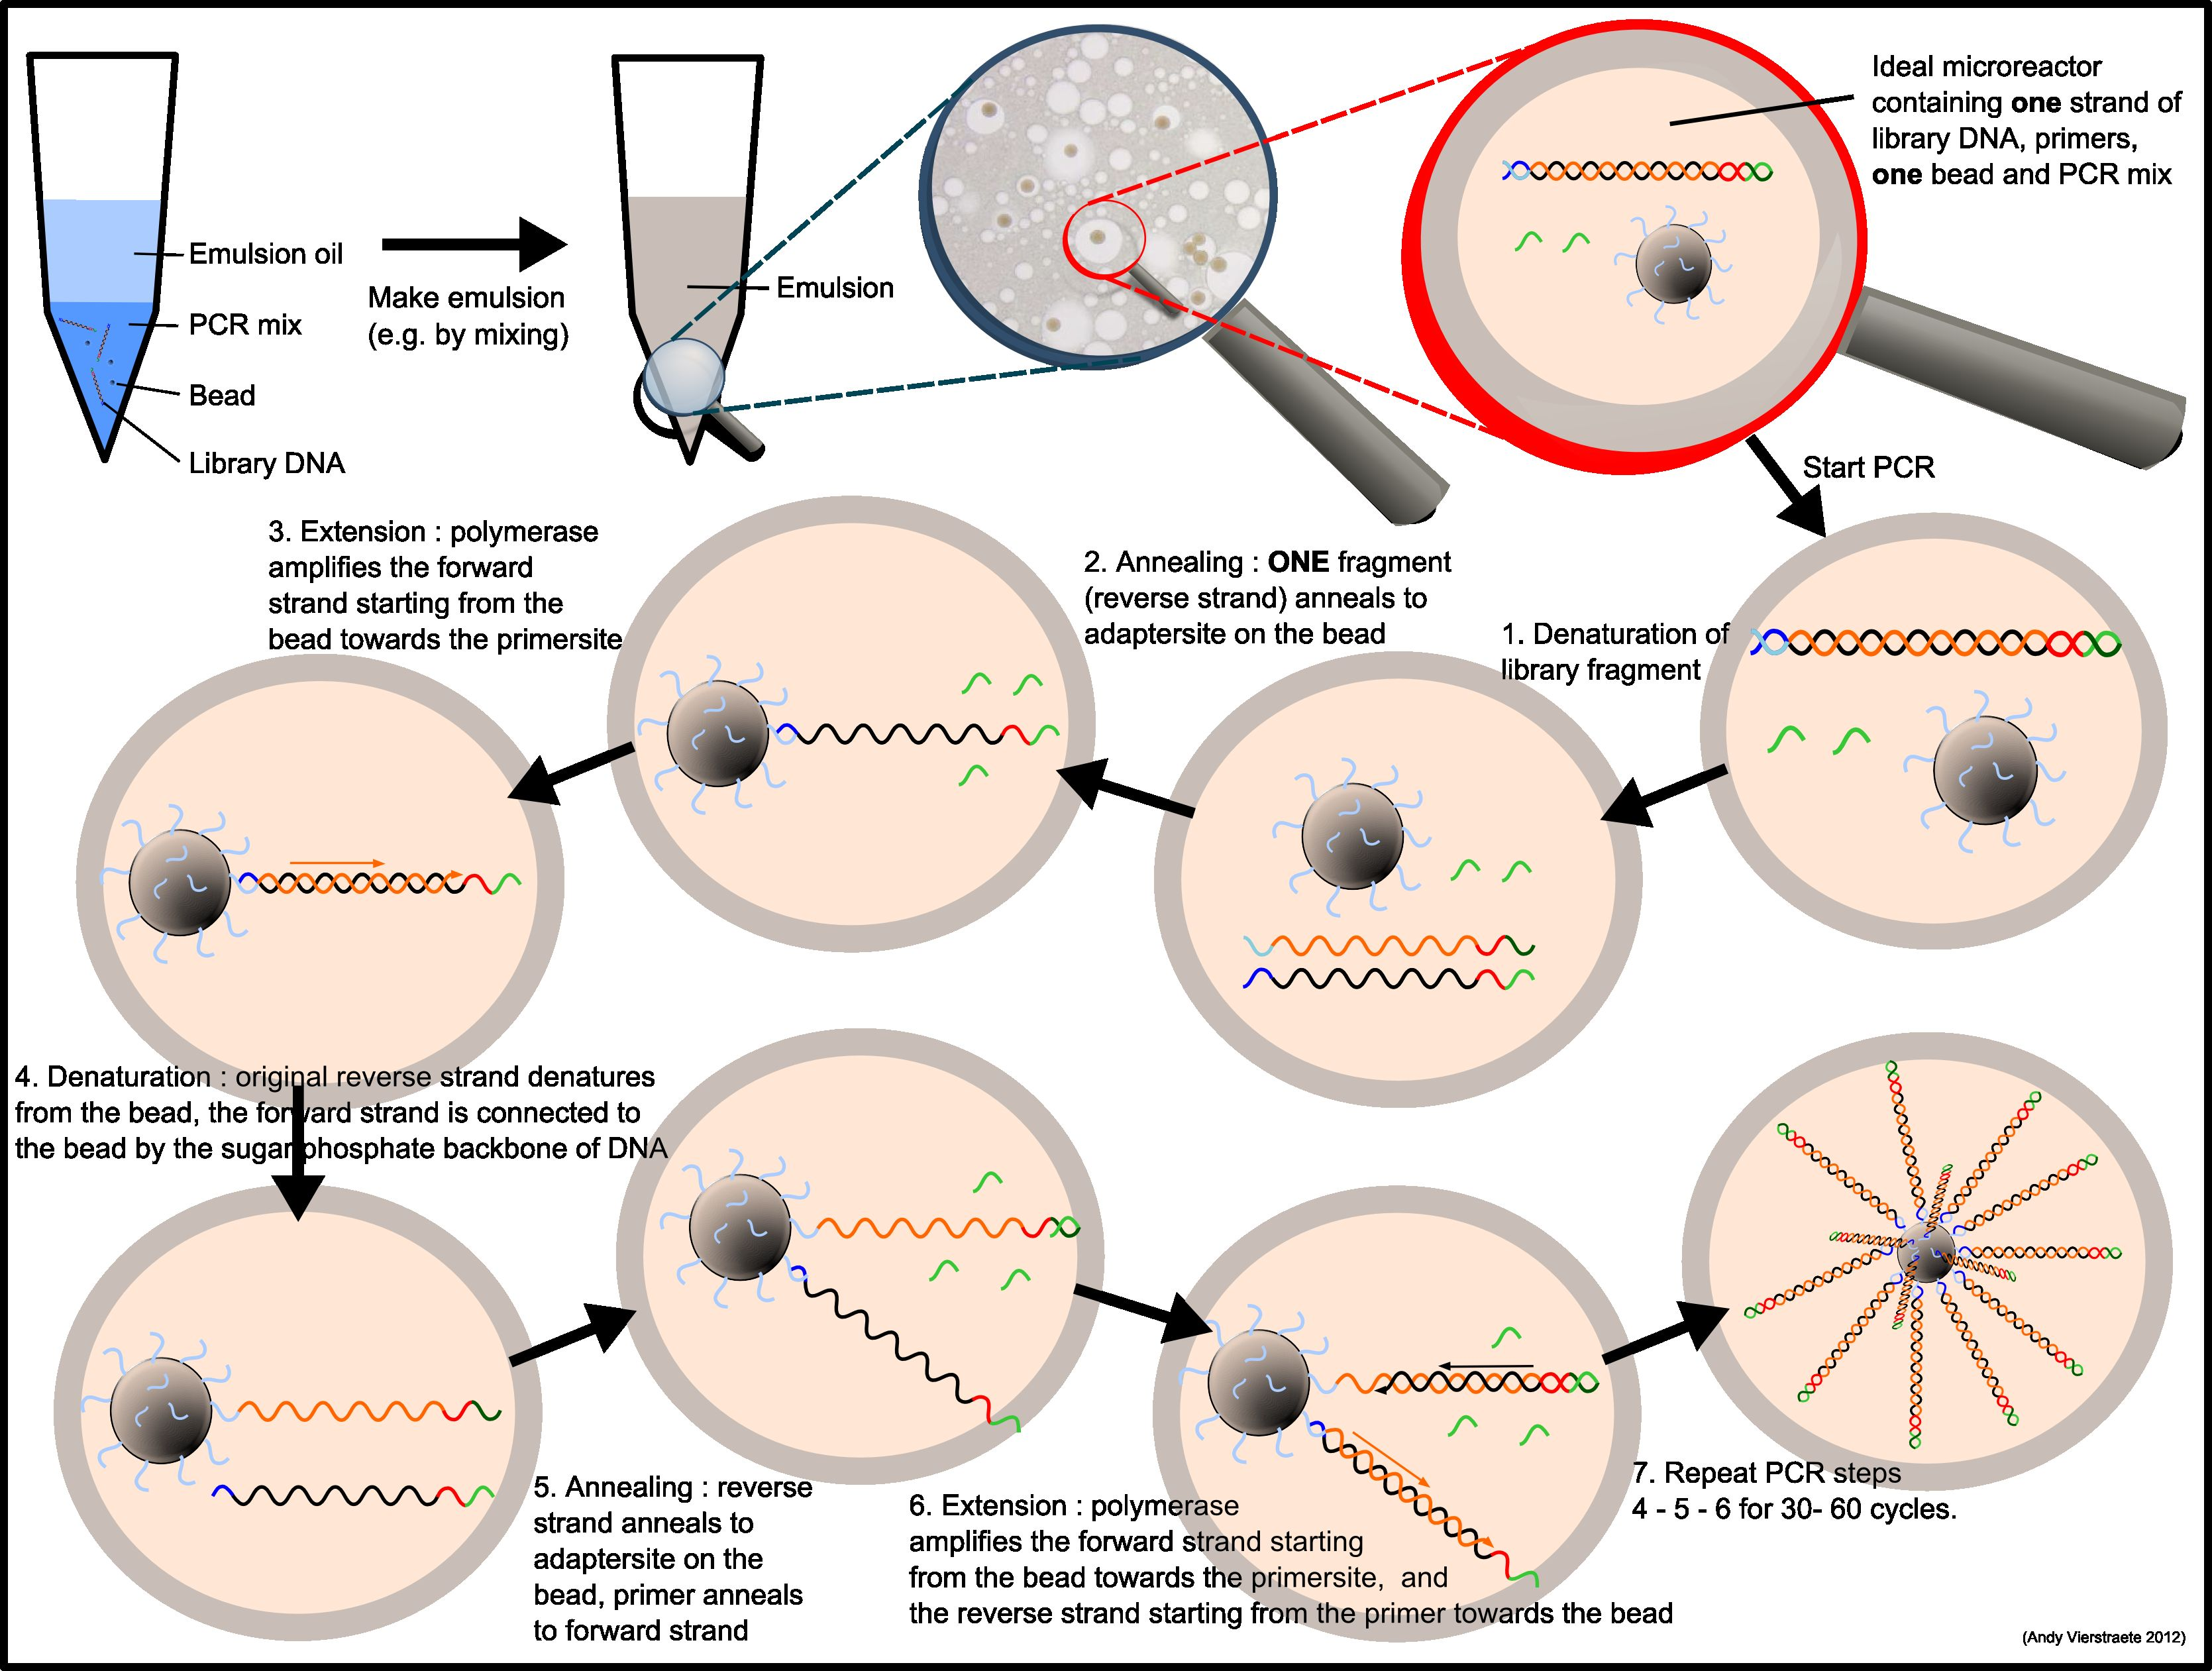
\includegraphics[scale=0.5]{emulsion}}
\caption{Emulsion PCR expliquée en détail2}
\end{figure}

\begin{figure}[!h]
\centering{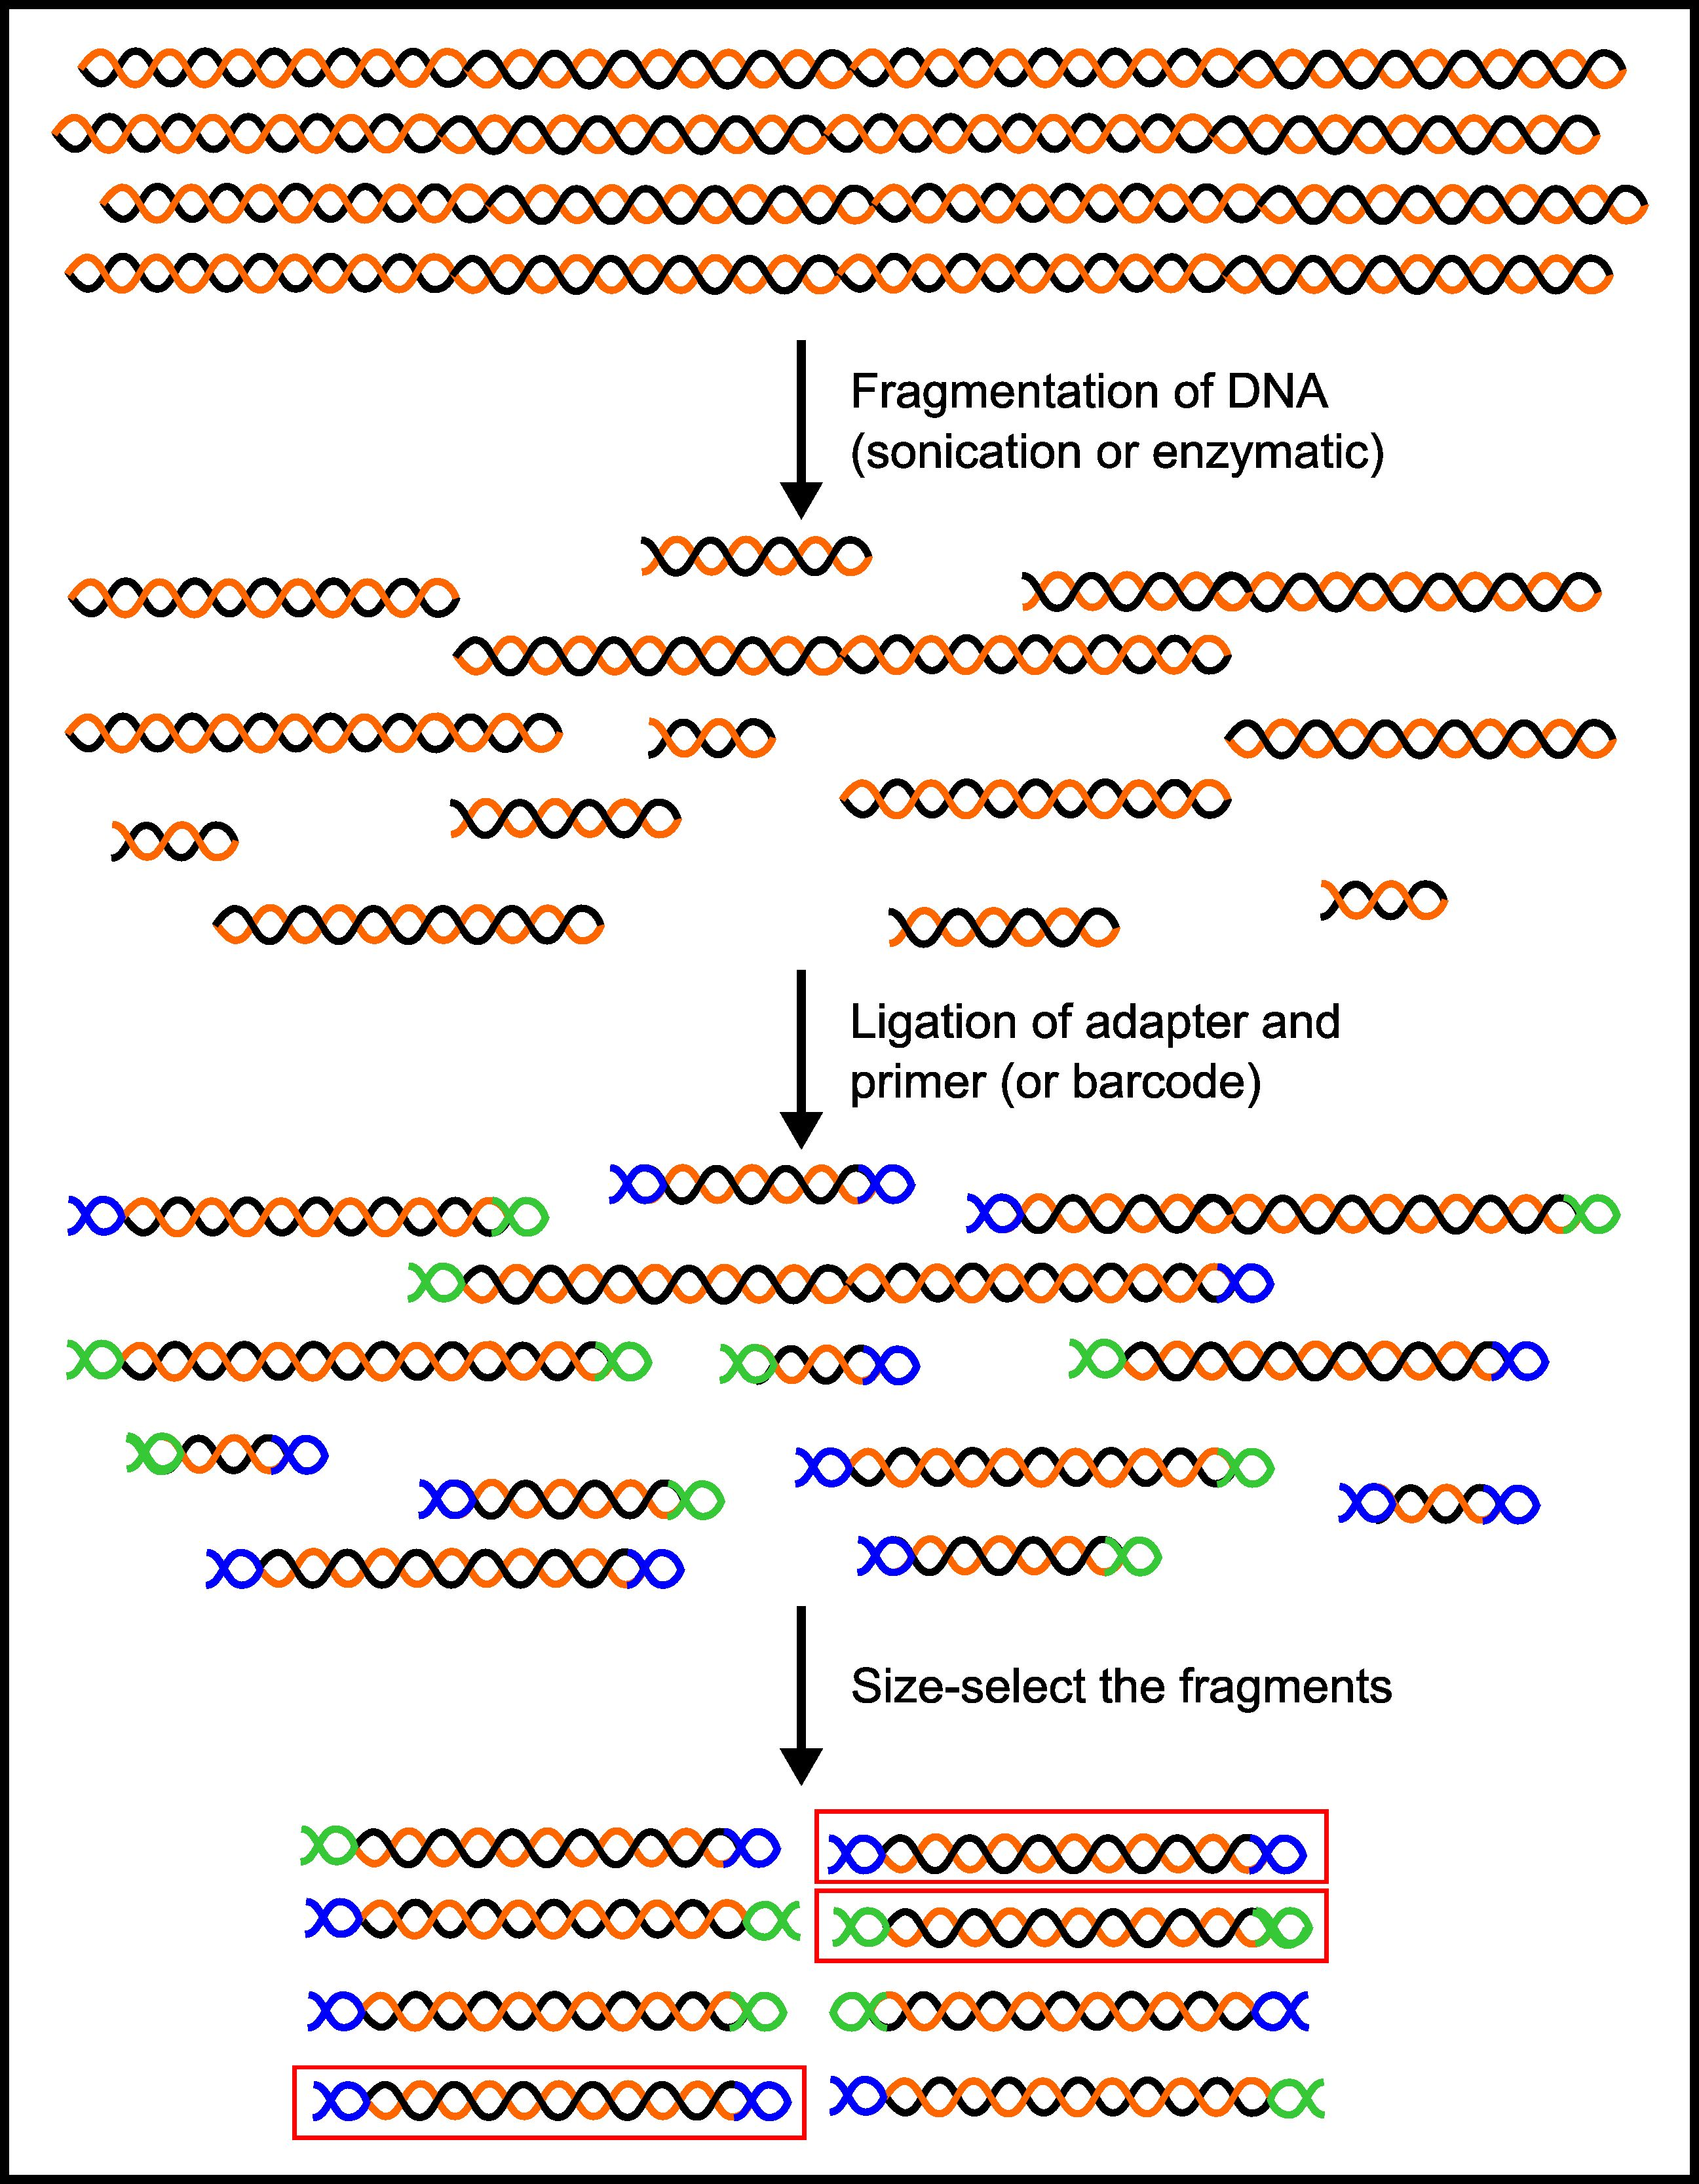
\includegraphics[scale=0.5]{2}}
\caption{Emulsion PCR expliquée en détail2}
\end{figure}

\begin{figure}[!h]
\centering{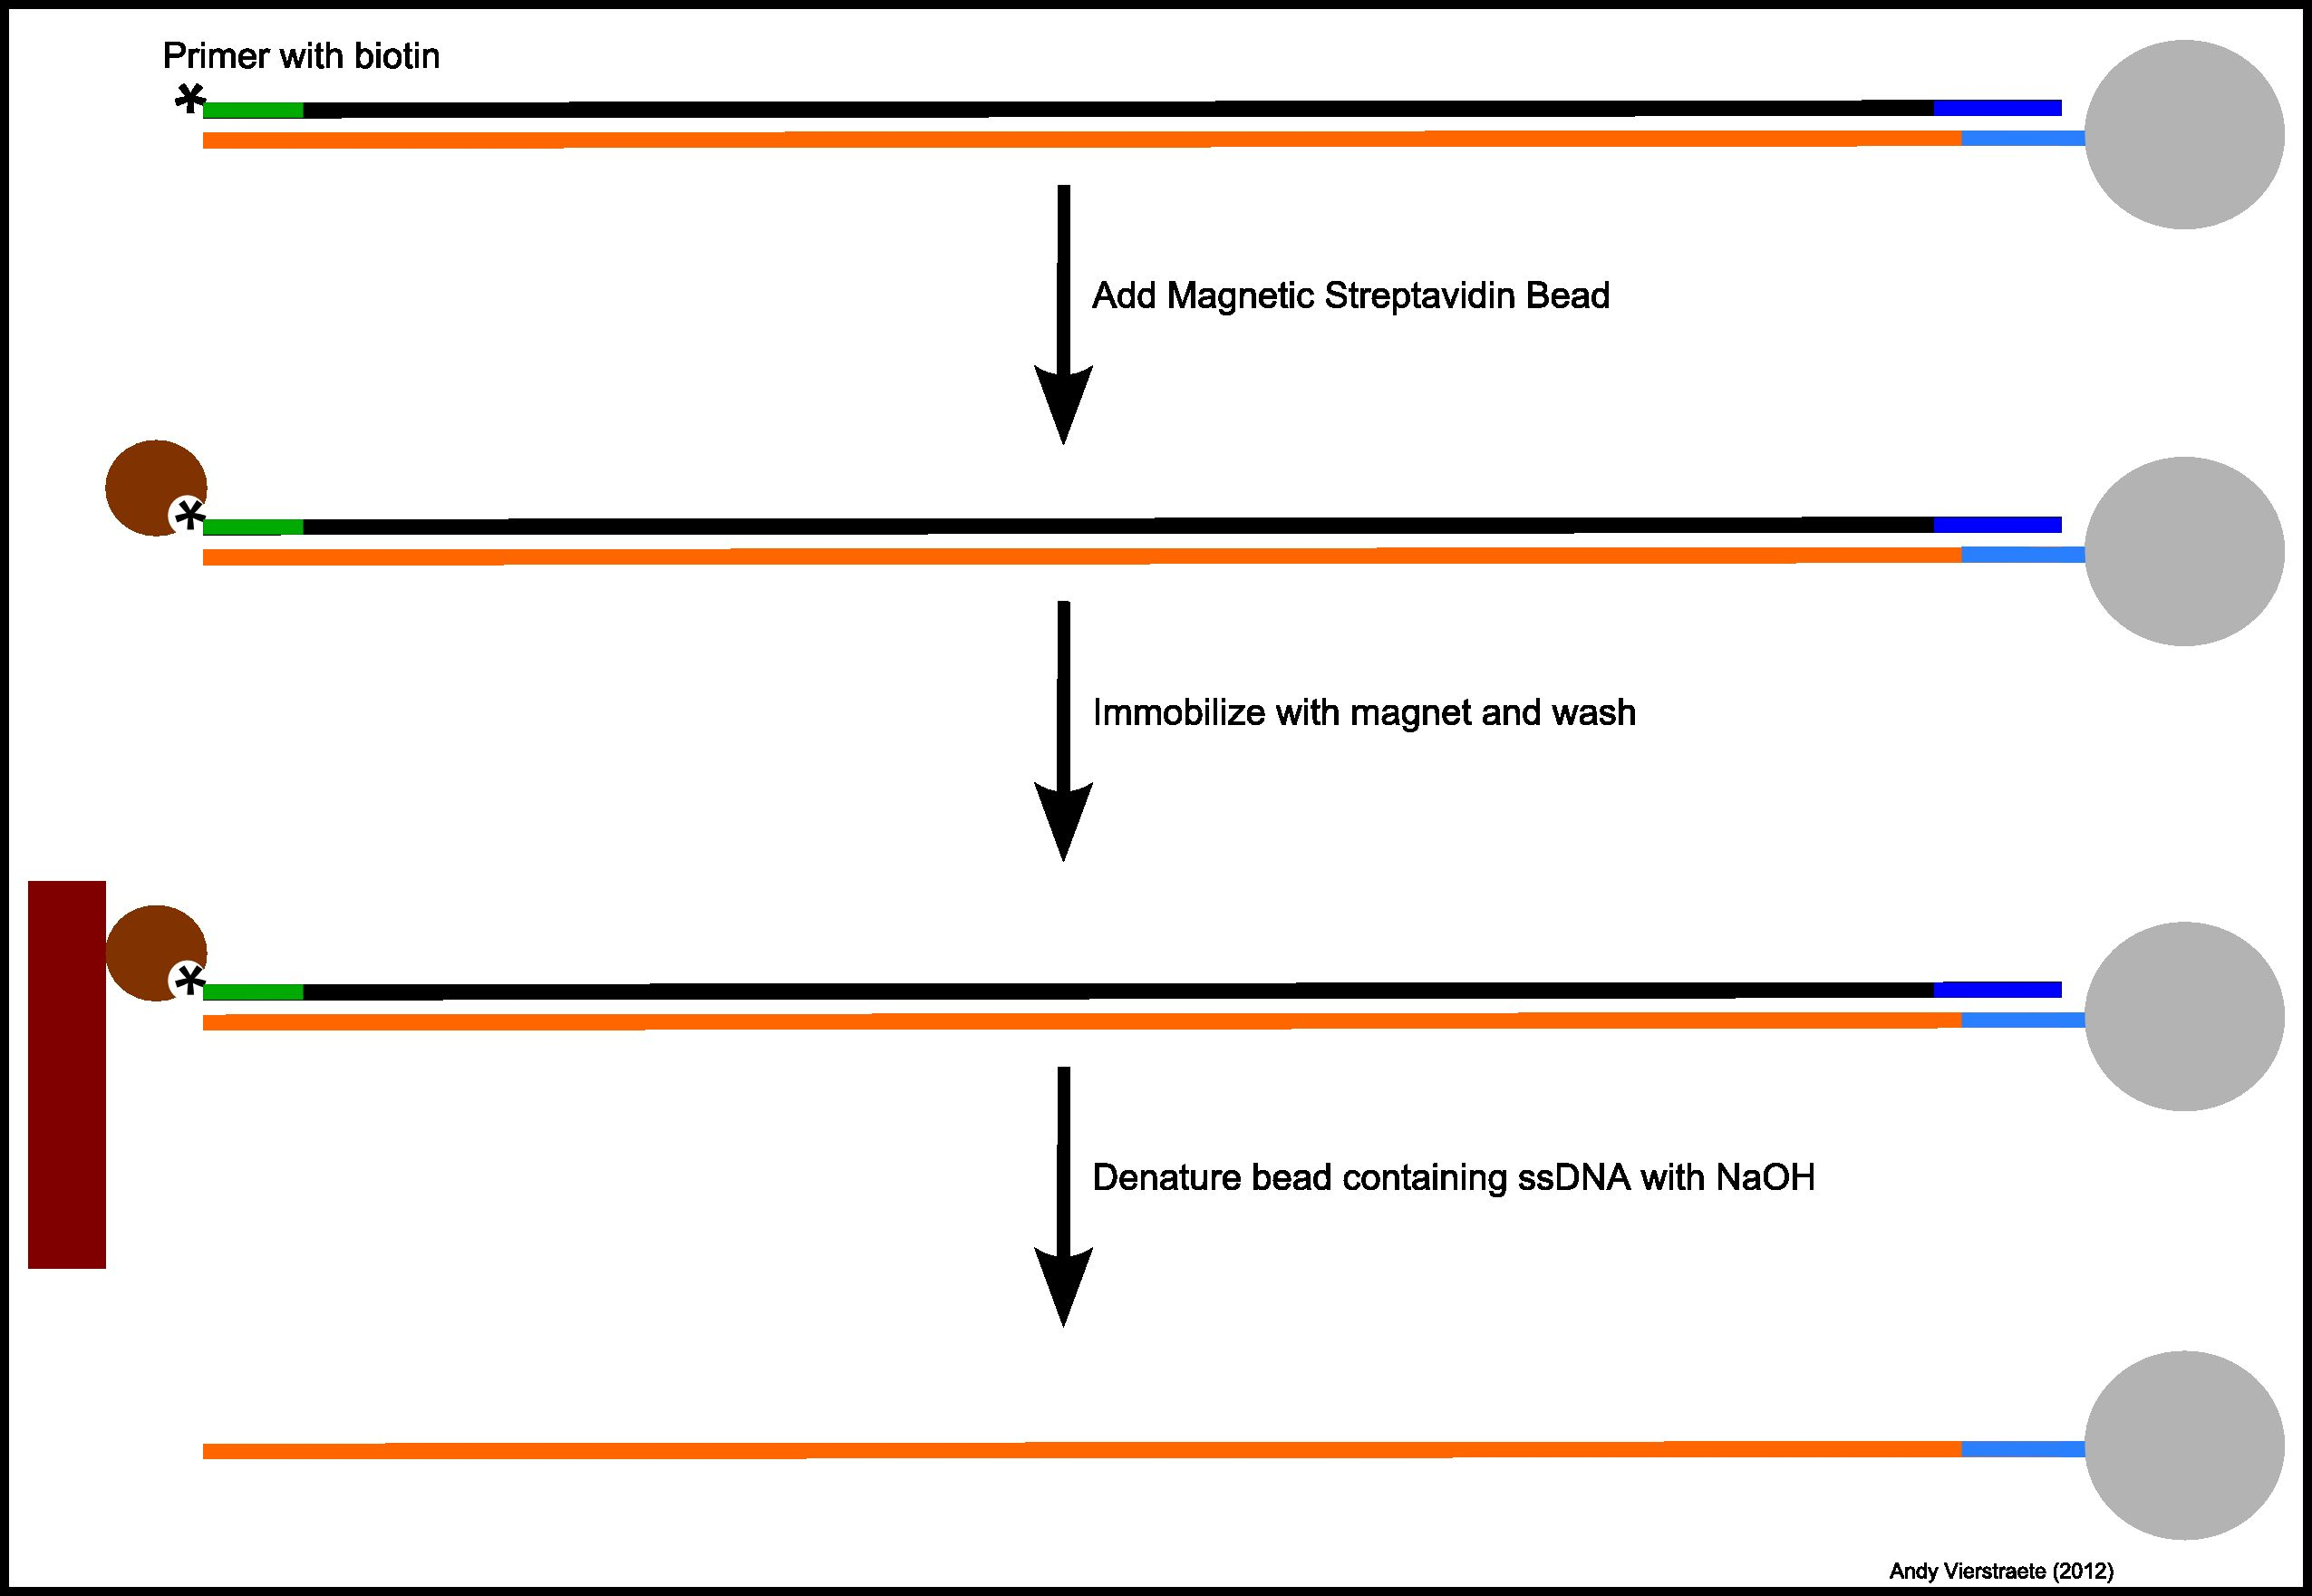
\includegraphics[scale=0.5]{3}}
\caption{Emulsion PCR expliquée en détail2}
\end{figure}

\begin{figure}[!h]
\centering{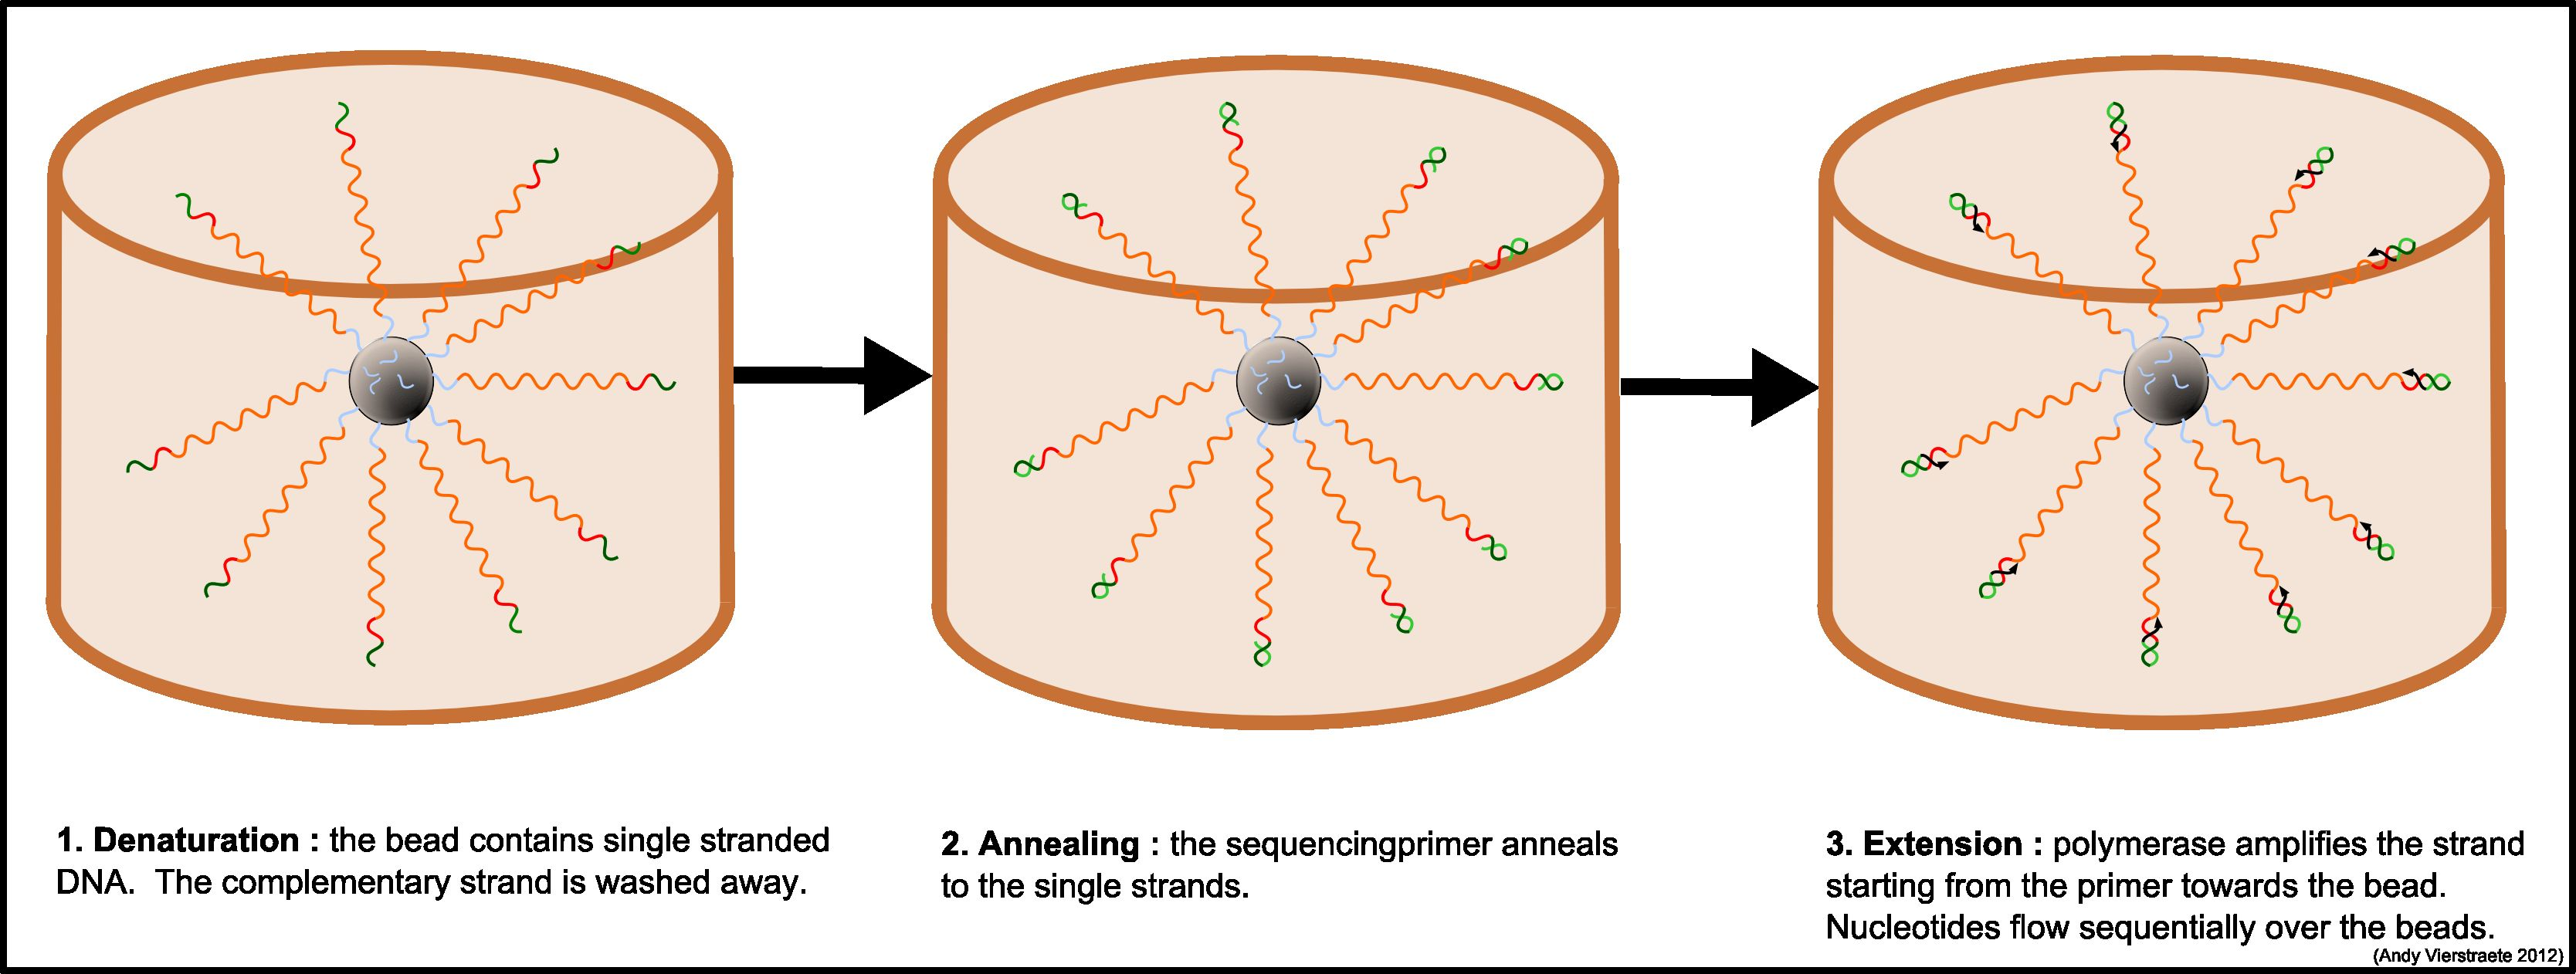
\includegraphics[scale=0.5]{4}}
\caption{Emulsion PCR expliquée en détail2}
\end{figure}

\begin{figure}[!h]
\centering{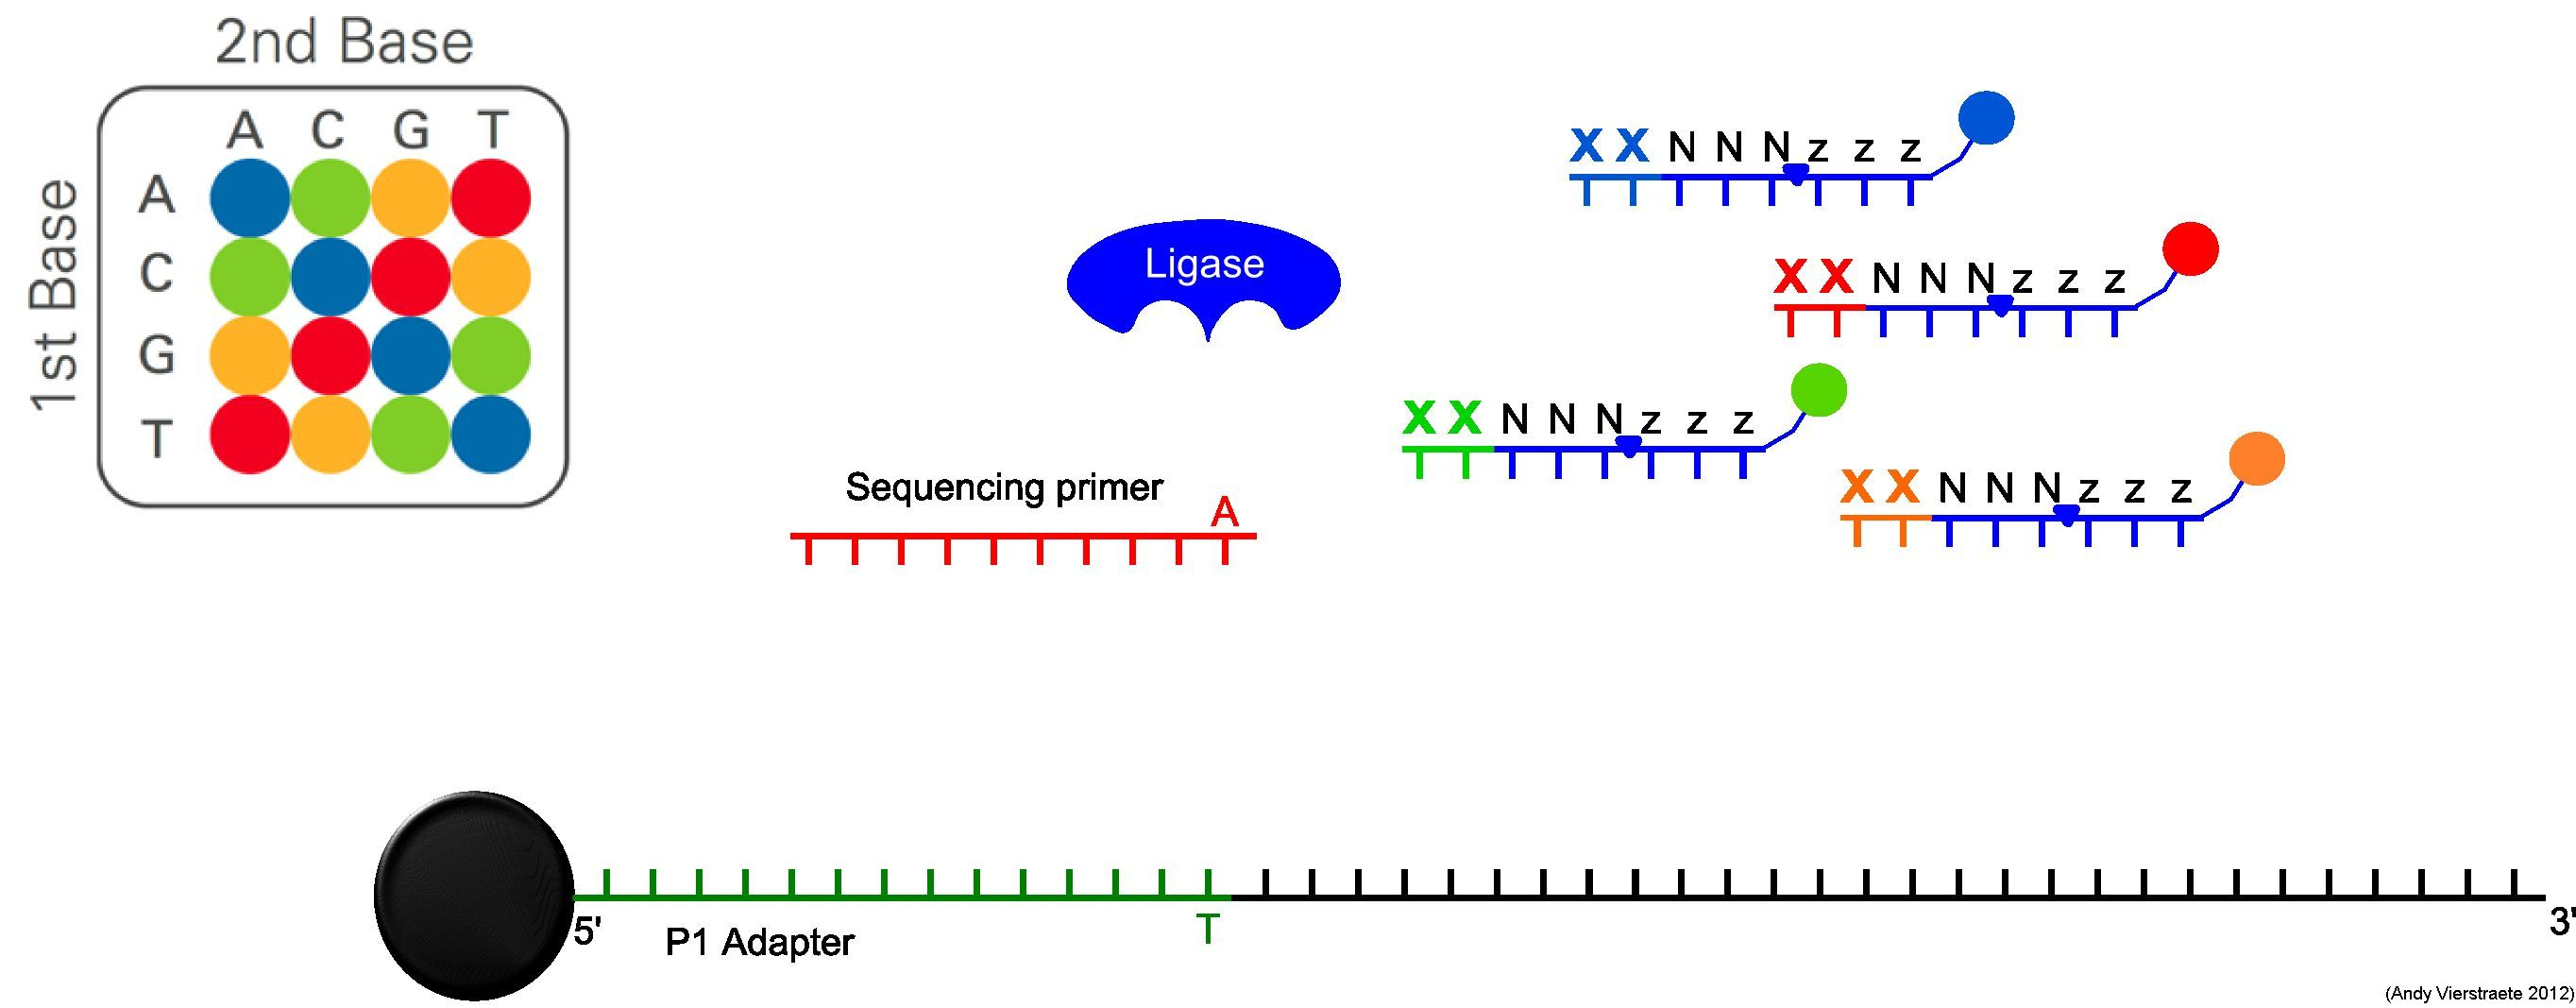
\includegraphics[scale=0.5]{5}}
\caption{Emulsion PCR expliquée en détail2}
\end{figure}

\begin{figure}[!h]
\centering{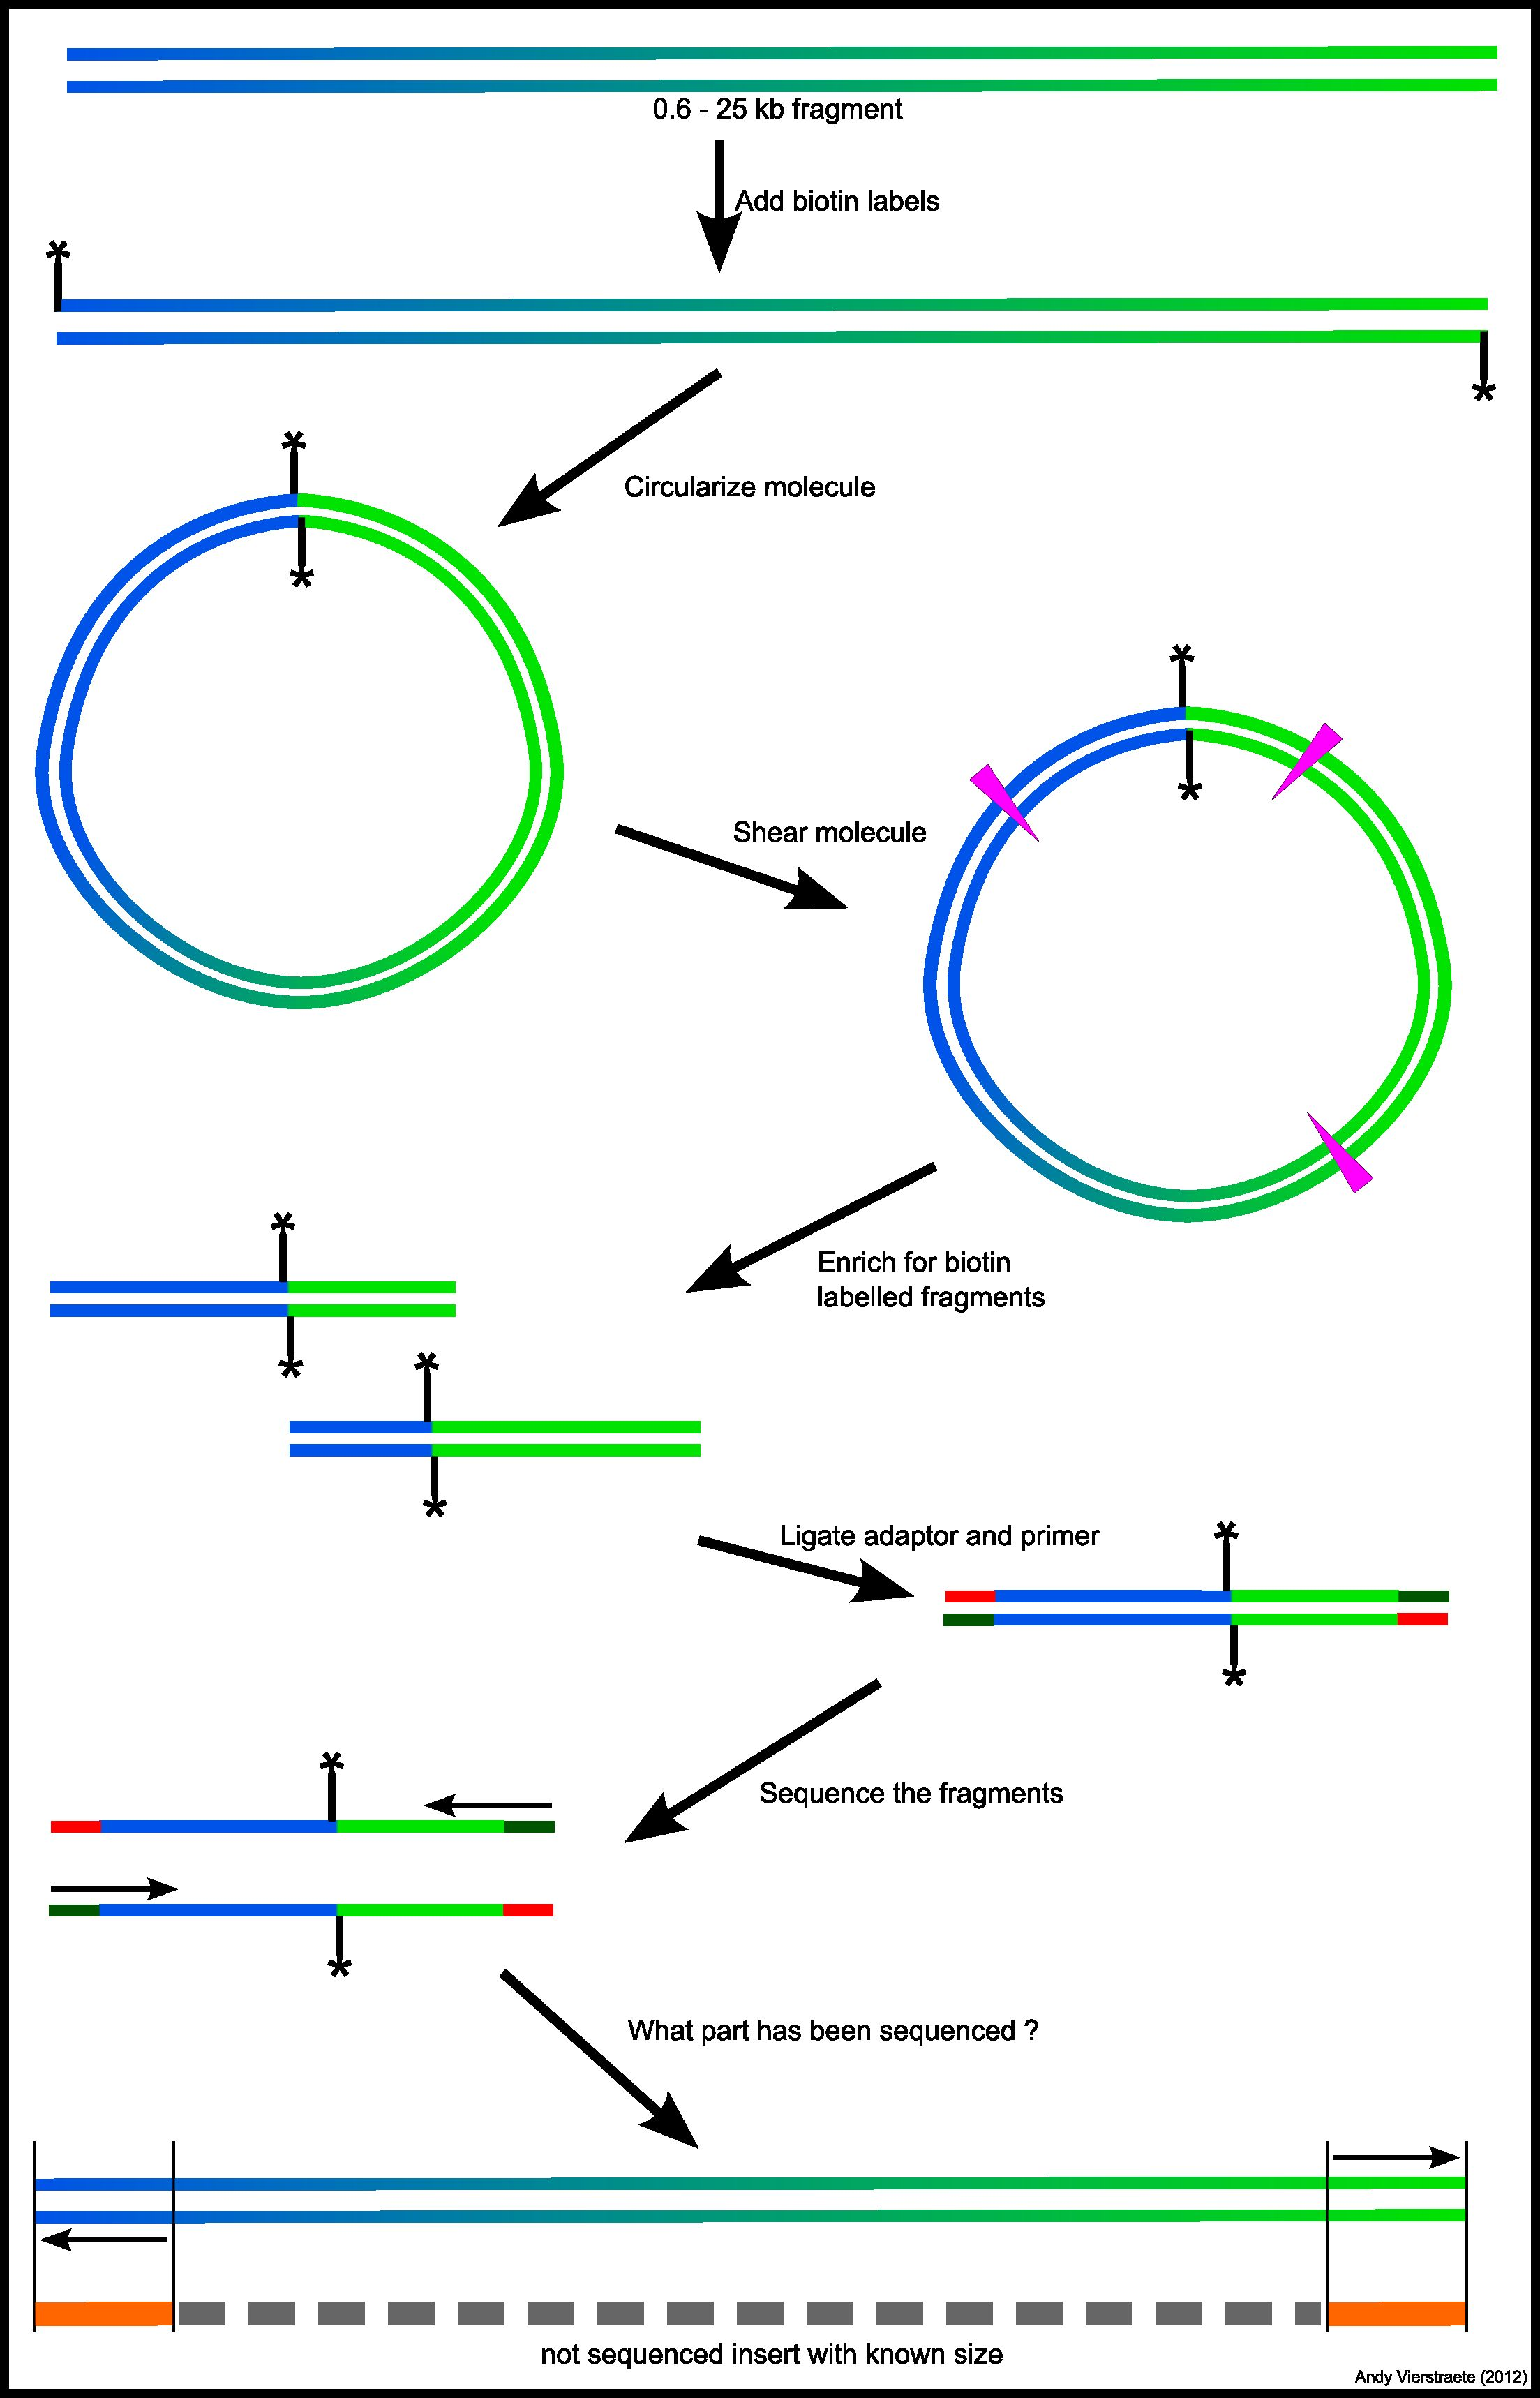
\includegraphics[scale=0.5]{6}}
\caption{Emulsion PCR expliquée en détail2}
\end{figure}

\section*{ANNEXE: Polony}

\begin{figure}[!h]
\centering{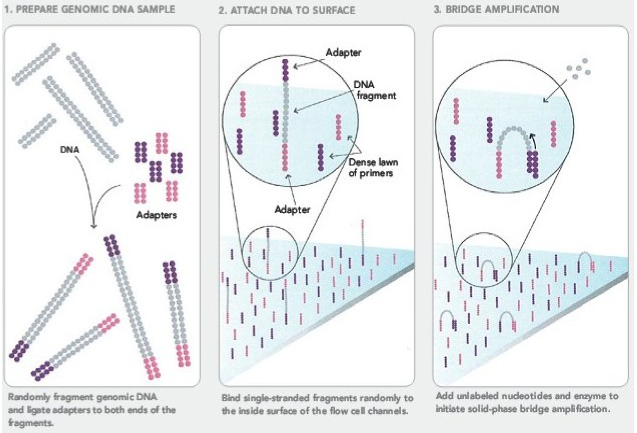
\includegraphics[scale=0.5]{polony1}}
\caption{Polony}
\end{figure}

\begin{figure}[!h]
\centering{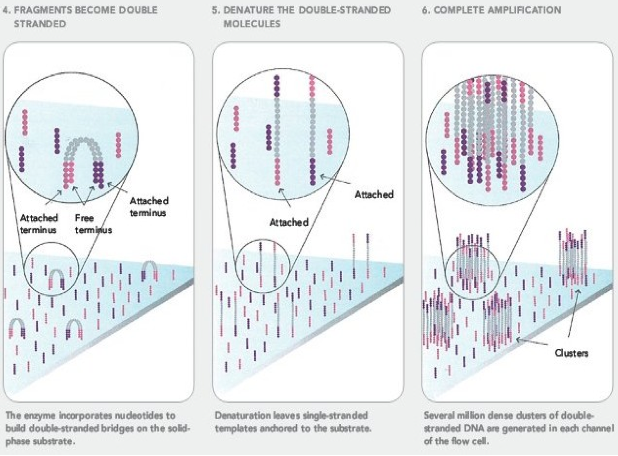
\includegraphics[scale=0.5]{polony2}}
\caption{Polony}
\end{figure}










\bibliographystyle{apalike}
\bibliography{Biblio2}
\end{document}


